\section{Individual Methods Summary \label{sec:individual_methods_summary}}

For the next experiments of this study, medium to high quality rank list are required.
In this chapter, we selected methods that can produce qualitative rank lists using different text representations.

Figure~\ref{fig:schema-rank_lists} contains a schema summarizing the steps to obtain rank lists using the different approaches.

The nine retained methods are presented in Table~\ref{tab:9rl}.
Four of them are using the $n$-MF tokens, two $n$-MF tokens $n$-grams, one compression techniques and two the $n$-POS with $n$-MF.

The complete evaluation of the rank list produced on these text representation for the three literary corpora are presented in Table~\ref{tab:rls_oxquarry_brunet}~and~\ref{tab:rls_st_jean} in annex.

\begin{figure*}
  \centering
  \caption{Rank lists methods schema}
  \label{fig:schema-rank_lists}
  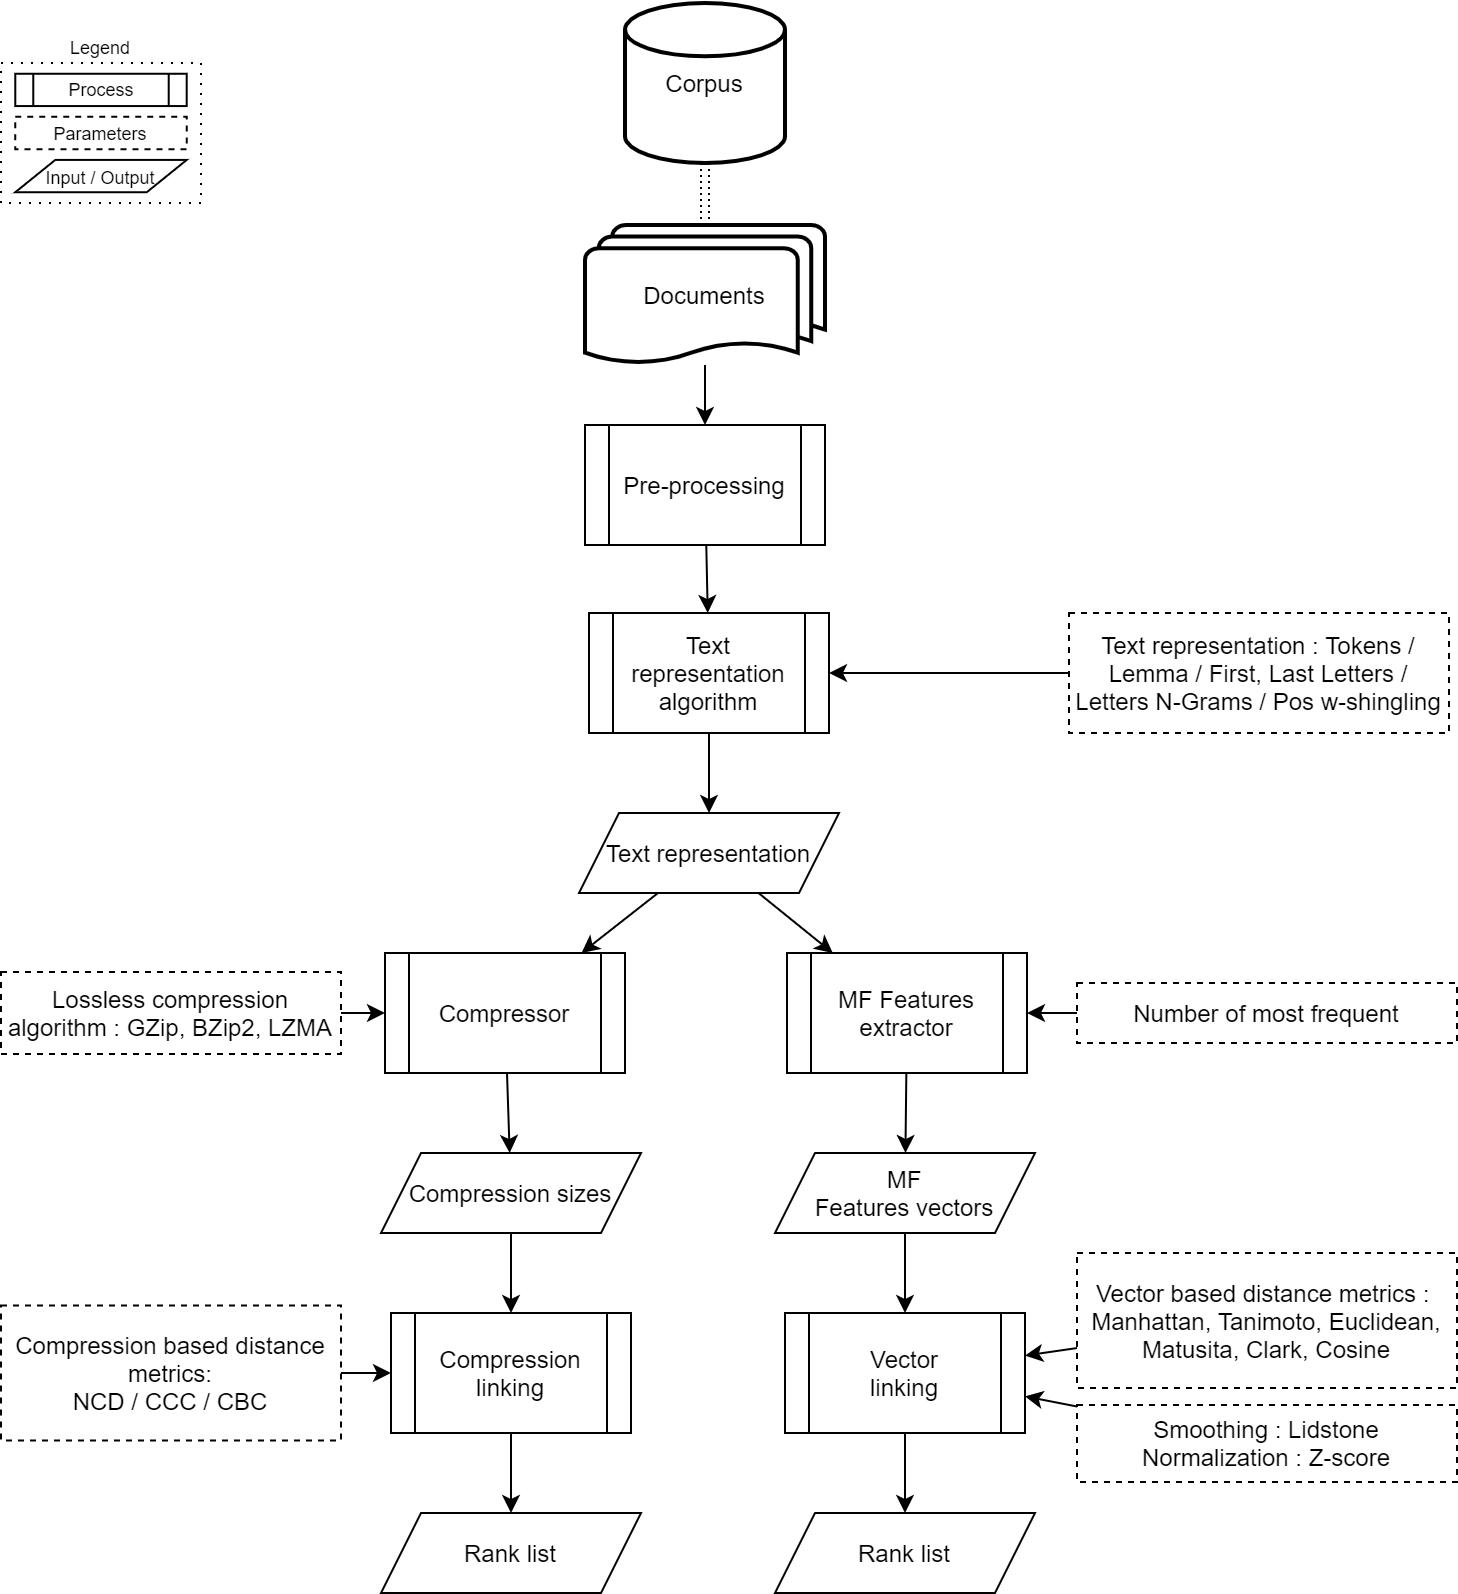
\includegraphics[width=0.90\linewidth]{img/schema-rank_lists.png}
\end{figure*}

\begin{table*}
  \centering
  \caption{Retained text representation and configuration}
  \label{tab:9rl}
  \begin{tabular}{c l l c c}
    \toprule
    Id &
    Text representation &
    Distance measure &
    Z-Score &
    Lidstone $\lambda$\\
    \midrule
    0 & $750$-MF tokens & Cosine Distance & Yes & $10^{-1}$\\
    1 & $750$-MF tokens & Clark & No & $10^{-1}$\\
    2 & $750$-MF tokens & Manhattan & Yes & $10^{-1}$\\
    3 & $750$-MF tokens & Tanimoto & No & $10^{-1}$\\
    4 & $3000$-MF tokens $3$-grams & Cosine distance & Yes & $10^{-1}$\\
    5 & $8000$-MF tokens $4$-grams & Cosine distance & Yes & $10^{-1}$\\
    6 & BZip2 compression & CBC distance & No & $10^{-1}$\\
    *7 & $250$-MF $2$-POS & Cosine distance & Yes & $10^{-1}$\\
    *8 & $1000$-MF $3$-POS & Manhattan distance & Yes & $10^{-1}$\\
    \bottomrule
  \end{tabular}

  \vspace{0.2cm}

  \textit{Note: text representation and configuration with a star (*) are only used for the St-Jean corpus.}\\
\end{table*}

\subsection{Distances' Matrix Visualization}

From a rank list, it is possible to create a distances' matrix (ref. Section~\ref{sec:distances_matrix}).
Distances' matrices created from rank list can be visualized.
To represent distances' matrices, each element of the matrix is mapped to a pixel in an 2D image.
The element value in the matrix is mapped to the pixel brightness.
The low values are in light colors and large values in dark colors

A good distance matrix should have each same author documents pair with a low distance (light color in the image) and different authors documents pairs with a large distance (dark color in the image).
The greater the contrast between the true links (same author documents) and the false links is (different authors documents), the better the distances' matrix is.

To better understand more easily this matrix, authors are sorted alphabetically.
If the distances' matrix can represent correctly the author style, same authors documents should have a low distance (light color in the image).
This should create light color squares in the diagonal.
The square size is related to the number of document written by this author.
The diagonal is the lightest color (white), since the distance between two same documents is always 0, with respect to the distance functions identity of indiscernible axiom.

The distance matrix for the best retained representation (the largerst AP) and the worse retained text representation (the lowest AP) is visually presented in Figure~\ref{fig:distances_matrix_oxquarry} for Oxquarry using a blue tint.
Respectively, the Clark distance on the $750$-MF which gives an average precision of $0.89$, and the Tanimito distance on the $750$-MF gives an $0.63$ average precision.
The diagonal is white in both images.
Light colors squares in the diagonal can clearly be observed on both distance matrix visualizations.
Some are slightly tainted, these documents pairs are harder to assert to be of a same authorship.

The Clark distance has overall a good distances matrix, except some document pairs from \textit{Conrad}, \textit{Hardy} and \textit{Orczy} which have darker colors, these are ranked below some false links in the rank list.

For Tanimoto, firstly one can observe these stripes, which are due to the max function in its computation, which create a more cleaved decision in the score value.

\begin{figure}
  \caption{Distance matrix visualization using Oxquarry}
  \label{fig:distances_matrix_oxquarry}

  \subcaption{Best retained text representation for Oxquarry ($750$-MF tokens with Clark)}
  \label{fig:distance_matrix_oxquarry_clark}
  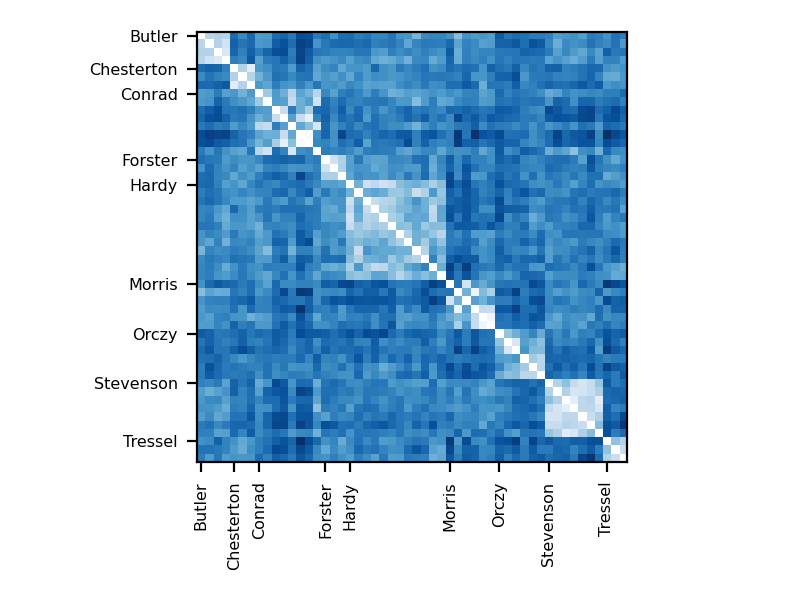
\includegraphics{img/distance_matrix_oxquarry_clark.png}

  \vspace{0.5cm}

  \subcaption{Worse retained text representation for Oxquarry ($750$-MF tokens with Tanimoto)}
  \label{fig:distance_matrix_oxquarry_tanimoto}
  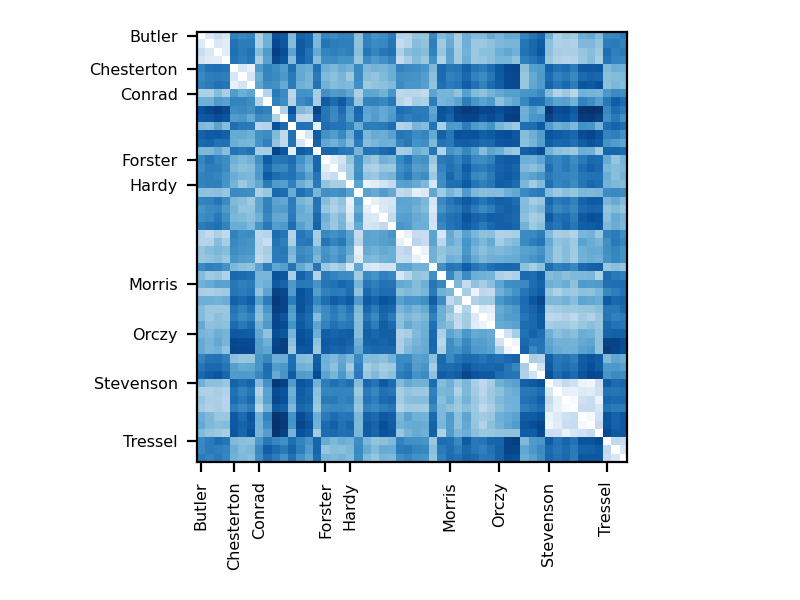
\includegraphics{img/distance_matrix_oxquarry_tanimoto.png}
\end{figure}

\subsection{Publication Date}

When dealing with false links ranked high in the rank list, as the previous experiment showed, some of these excerpt pairs use similar words (ref. Section~\ref{sec:frequent_errors}).
These shared words might be related to the era the book was written in.
The following experiment tries to investigate on this assumption.
We try to verify this assumption by analyzing the difference in publication date for the most incorrect document pairs in the rank lists (false links ranked high in the rank list).

In the St-Jean corpus publication paper, the publication dates of each excerpt are available~\cite{st_jean}.
First, the publication date distribution of the corpus must be understood.
Figure~\ref{fig:dates_distribution} show the distribution of the publication date in the St-Jean corpus.
The corpus mainly focus on the two last thirds of the XIX century, only a few books are published between 1800 and 1830.

The date difference distribution for each pair of documents can be computed.
Figure~\ref{fig:dates_differences_true_false} shows the date difference distribution for the true and false links.
The union of both of them represent every possible document pairs (the whole rank list), in this figure the bars are stacked to represent every link.
Table~\ref{tab:date_differences} shows statistics on the distributions.

True links have a low mean date difference of $5.11$ years with a standard deviation of $7.05$ years.
This low mean can be explained by the fact that most authors in the St-Jean corpus have excerpts from the same book.
Also, the authors publish their books during their career, which is limited to their active years (life span minus early stages and old age for most authors).
In fact, $281$ of the $670$ ($\sim 42\%$) true links are excerpts published the same year.
$453$ out of $670$ ($\sim 68\%$) true links have a publication date difference below or equal to $5$ years.

For St-Jean the largest date difference from the same author (correspond to the longest career in the corpus) is $31$ years, which correspond to the two following books from Victor Hugo: \textit{Notre Dame de Paris} (The Hunchback of Notre-Dame), in 1831 and \textit{Les Misérables}, in 1862.

The average date difference for the false links is $28.24$ years, with a standard deviation of $20.73$ years.
The overall average (both true and false links) is at $29.04$ years, with a standard deviation of $20.58$ years.

The previous statistics can be compared to the ones in Figure~\ref{fig:dates_differences_r_false}.
This figure shows the date difference density on the top-r false links (r is chosen at 670, it corresponds to the number of true links in St-Jean) in a rank list.
The rank list used have an average precision of $85\%$.
It is obtained by the Z-Score fusion of the retained text representations (Table~\ref{tab:rls_st_jean}, ref. Chapter~\ref{sec:fusions}).

Two interesting information can be extracted here.
Firstly, the mean is lower by $7.75$ years ($29.04$ - $21.29$) compared to every false links and have a narrow standard deviation distribution.
Having a lower mean in this case indicate that more mistakes are made for document pairs with a lower date difference then for the ones with a large date difference, which can lead to the following conclusion: distinguishing between a false link and a true link for documents pair with low date difference is harder.
Secondly, we can observe a drop after $35$ years of date difference, which indicate that links in the interval $\left[0-35\right]$ years are harder to discriminate between a true link and a false link than the ones outside this interval.

The 35 years interval can be related to the generation factor, the age of woman giving birth is around 25-34 in France~\cite{generations}, authors' birth country for this corpus.
Each new generation tends to use its own vocabulary, and thus it can be harder to discriminate the author of text belonging to the same generation, if we assume that the authors write their books at around the same age.
In the other hand, having different vocabulary can indicate a different time period and can be used to detect document forgery~\cite{savoy_stylo}.

The small spike between 60 and 65 in the top-r false link is due to the matching of most excerpts from \textit{Volupté} (excerpts 117, 135, 151, 165, 181, 189) written by Charles Sainte-Beuve in 1834 and \textit{Les plaisirs et les jours} (excerpts 114, 132, 148) written by Marcel Proust in 1896.
Out of the 18 possible false link for these excerpts, 12 are in the top-r false link.
This indicates that the styles used in these two books are close.
We can not discriminate the authors correctly even though the books were published with 62 years interval.
This interesting observation could be further discussed with a historian specialized in literature.

\begin{figure}
  \centering
  \caption{Dates distribution and date differences distribution on St-Jean}

  \subcaption{Dates distribution}
  \label{fig:dates_distribution}
  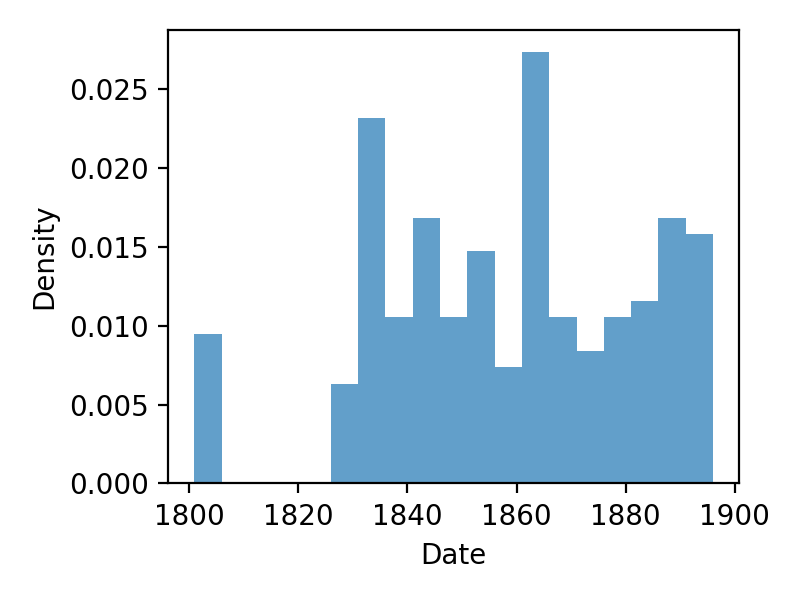
\includegraphics[width=\linewidth]{img/dates_distribution.png}

  \vspace{0.5cm}

  \subcaption{True and false links date differences distribution}
  \label{fig:dates_differences_true_false}
  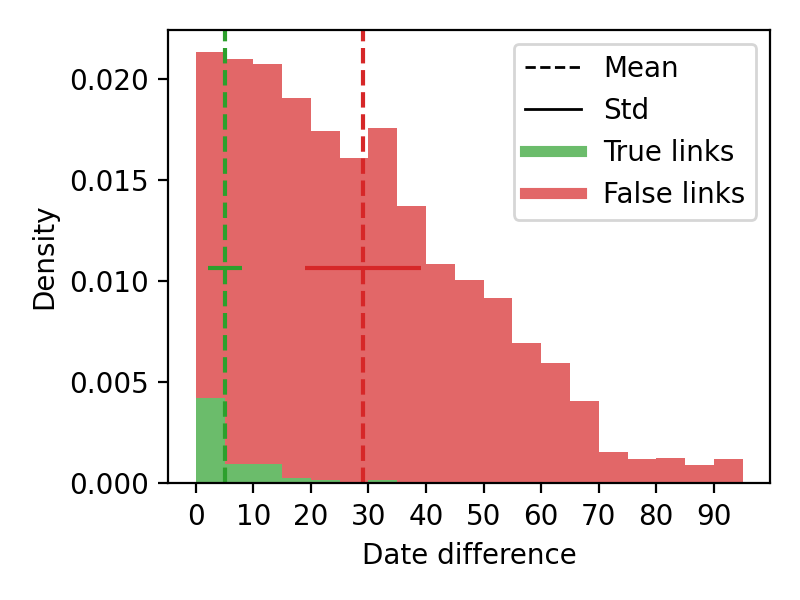
\includegraphics[width=\linewidth]{img/dates_differences_true_false.png}

  \vspace{0.5cm}

  \subcaption{Top-r false links using a rank list with 85\% average precision}
  \label{fig:dates_differences_r_false}
  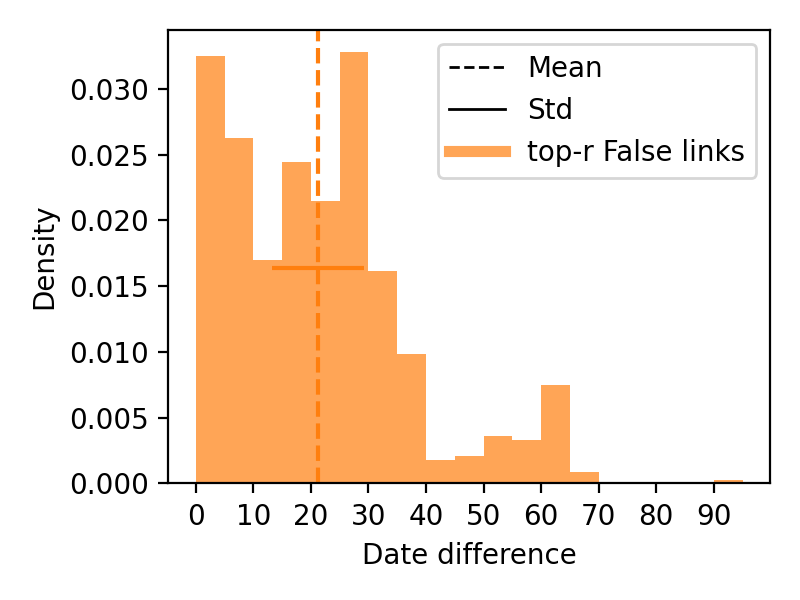
\includegraphics[width=\linewidth]{img/dates_differences_r_false.png}
\end{figure}

\begin{table}
  \centering
  \caption{Date differences statistics}
  \label{tab:date_differences}
    \begin{tabular}{l r r}
      \toprule
      Links                & Mean  & Std   \\
      \midrule
      True links           &  5.11 &  7.06 \\
      False links          & 29.04 & 20.58 \\
      True and False links & 28.24 & 20.73 \\
      top-r False links    & 21.29 & 16.00 \\
      \bottomrule
    \end{tabular}
\end{table}
